
% This LaTeX was auto-generated from MATLAB code.
% To make changes, update the MATLAB code and republish this document.

\documentclass{article}
\usepackage{graphicx}
\usepackage{color}

\sloppy
\definecolor{lightgray}{gray}{0.5}
\setlength{\parindent}{0pt}

\begin{document}

    
    
\subsection*{Contents}

\begin{itemize}
\setlength{\itemsep}{-1ex}
   \item Analyze Sensitivity
   \item Plot Histograms
   \item Error spread
   \item Exit information for error-minimizing experiment
   \item Plot Incidence and Prevalence of error minimizing
\end{itemize}


\subsection*{Analyze Sensitivity}

\begin{verbatim}
%{
A few tools to analyze the results following sensitivity analysis.

1. Histogram of optimal values
2. Error vs iteration.
3.
%}
\end{verbatim}
\begin{verbatim}
imageName = 'Run16v2';

NumSims=size(XX,1);
numSims = NumSims;


allq1 = zeros(NumSims,1);
allq2 = zeros(NumSims,1);
allX0 = zeros(NumSims,1);
allE0 = zeros(NumSims,1);
allL0 = zeros(NumSims,1);
allR0 = zeros(NumSims,1);

for i=1:NumSims
    currentx = XX{i,2};
    allq1(i)=currentx(1);
    allq2(i) = currentx(2);
    allX0(i) = currentx(3);
    allE0(i) = currentx(4);
    allL0(i) = currentx(5);
    allR0(i) = currentx(6);
end

numbins=20;
\end{verbatim}


\subsection*{Plot Histograms}

\begin{verbatim}
figure(1)

subplot(2,3,1)

% histfit(allq1,numbins)
histfit(allq1,numbins)
title('Distribution of optimal q1')

subplot(2,3,2)
histfit(allq2,numbins)
title('Distribution of optimal q2')


subplot(2,3,3)
histfit(allE0,numbins)
title('Distribution of optimal X0')

subplot(2,3,4)
histfit(allE0,numbins)
title('Distribution of optimal E0')

subplot(2,3,5)
histfit(allL0,numbins)
title('Distribution of optimal L0')

subplot(2,3,6)
histfit(allR0,numbins)
% histfit(allR0,numbins)
title('Distribution of optimal R0')
saveas(gcf,['Optimized parameter distribution across sensitivity analysis',imageName, '.png'])
\end{verbatim}

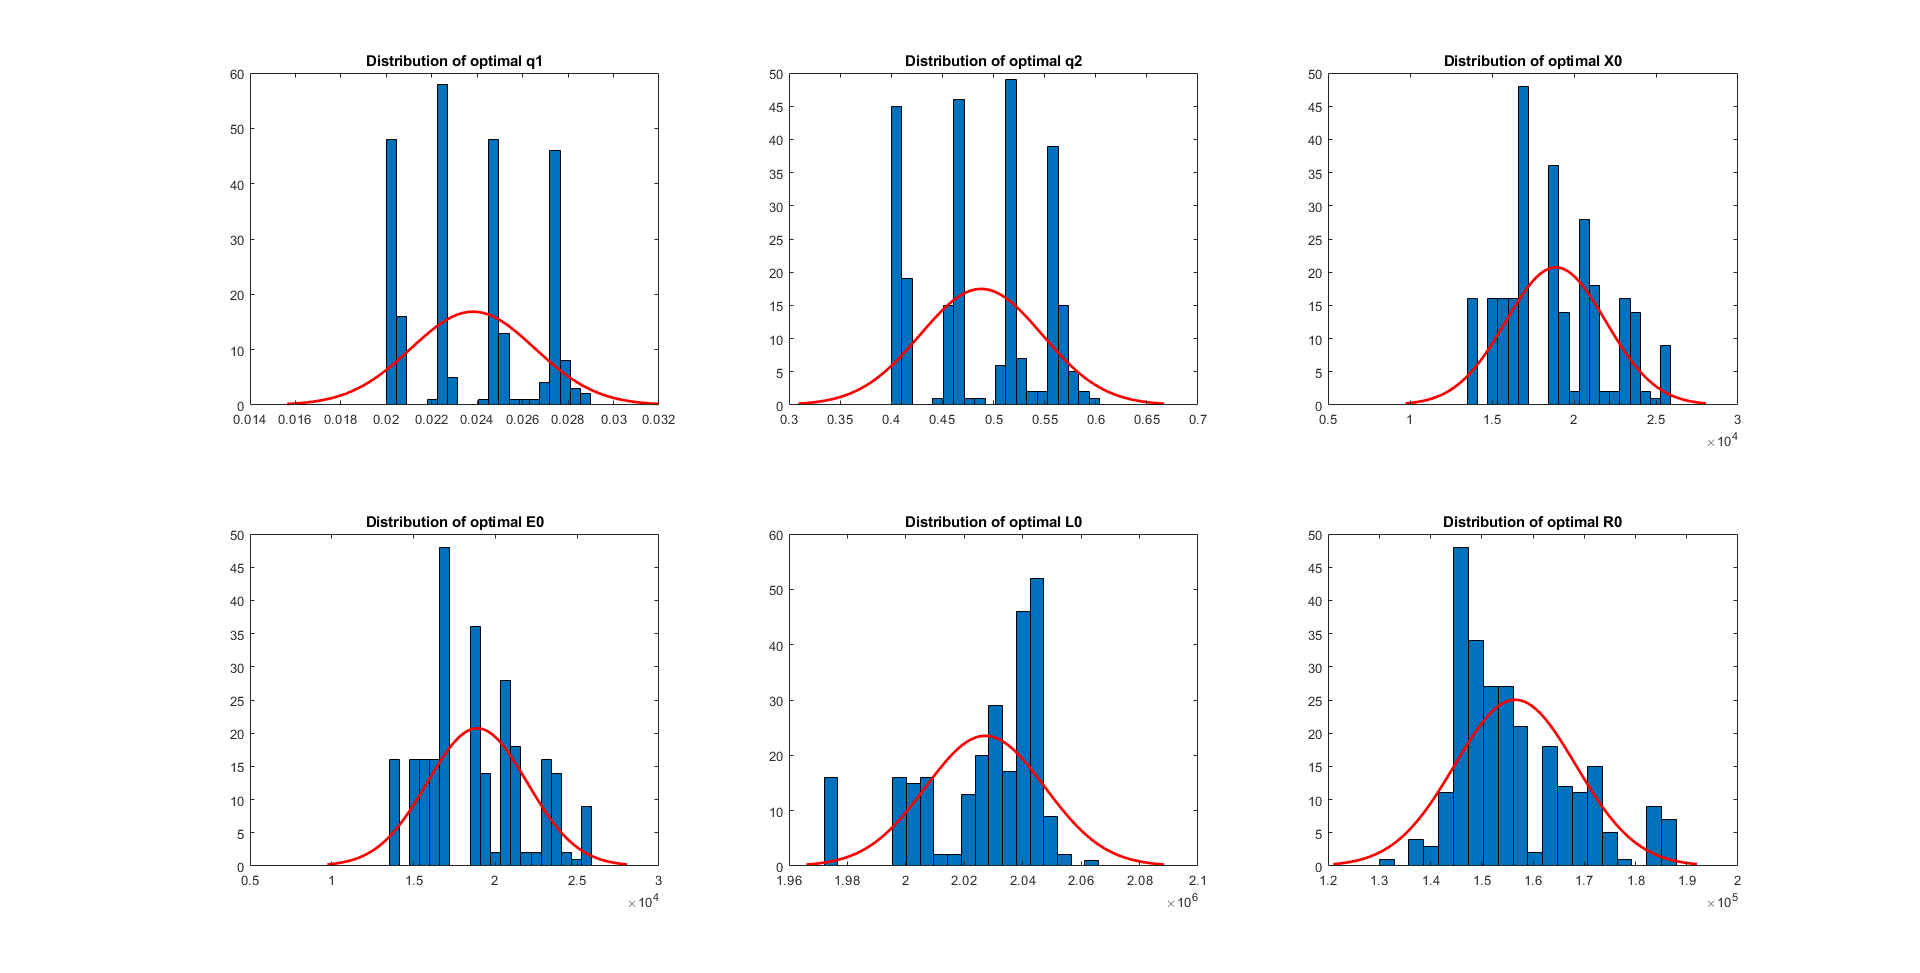
\includegraphics [width=4in]{analyze_Sensitivity_01.png}


\subsection*{Error spread}

\begin{verbatim}
% numSims = size(XX,1);

errors = zeros(numSims,1);
for k=1:numSims
    errors(k) = XX{k,6};
end

figure(2)
plot(errors)
title('Error vs experiment')

display(['The standard deviation of error is ',num2str(std(errors))])
display(['The min and max error are respectively ', num2str(min(errors)), ' ', num2str(max(errors)) ])
\end{verbatim}

        \color{lightgray} \begin{verbatim}The standard deviation of error is 5.1869e-05
The min and max error are respectively 5.8434 5.8437
\end{verbatim} \color{black}
    
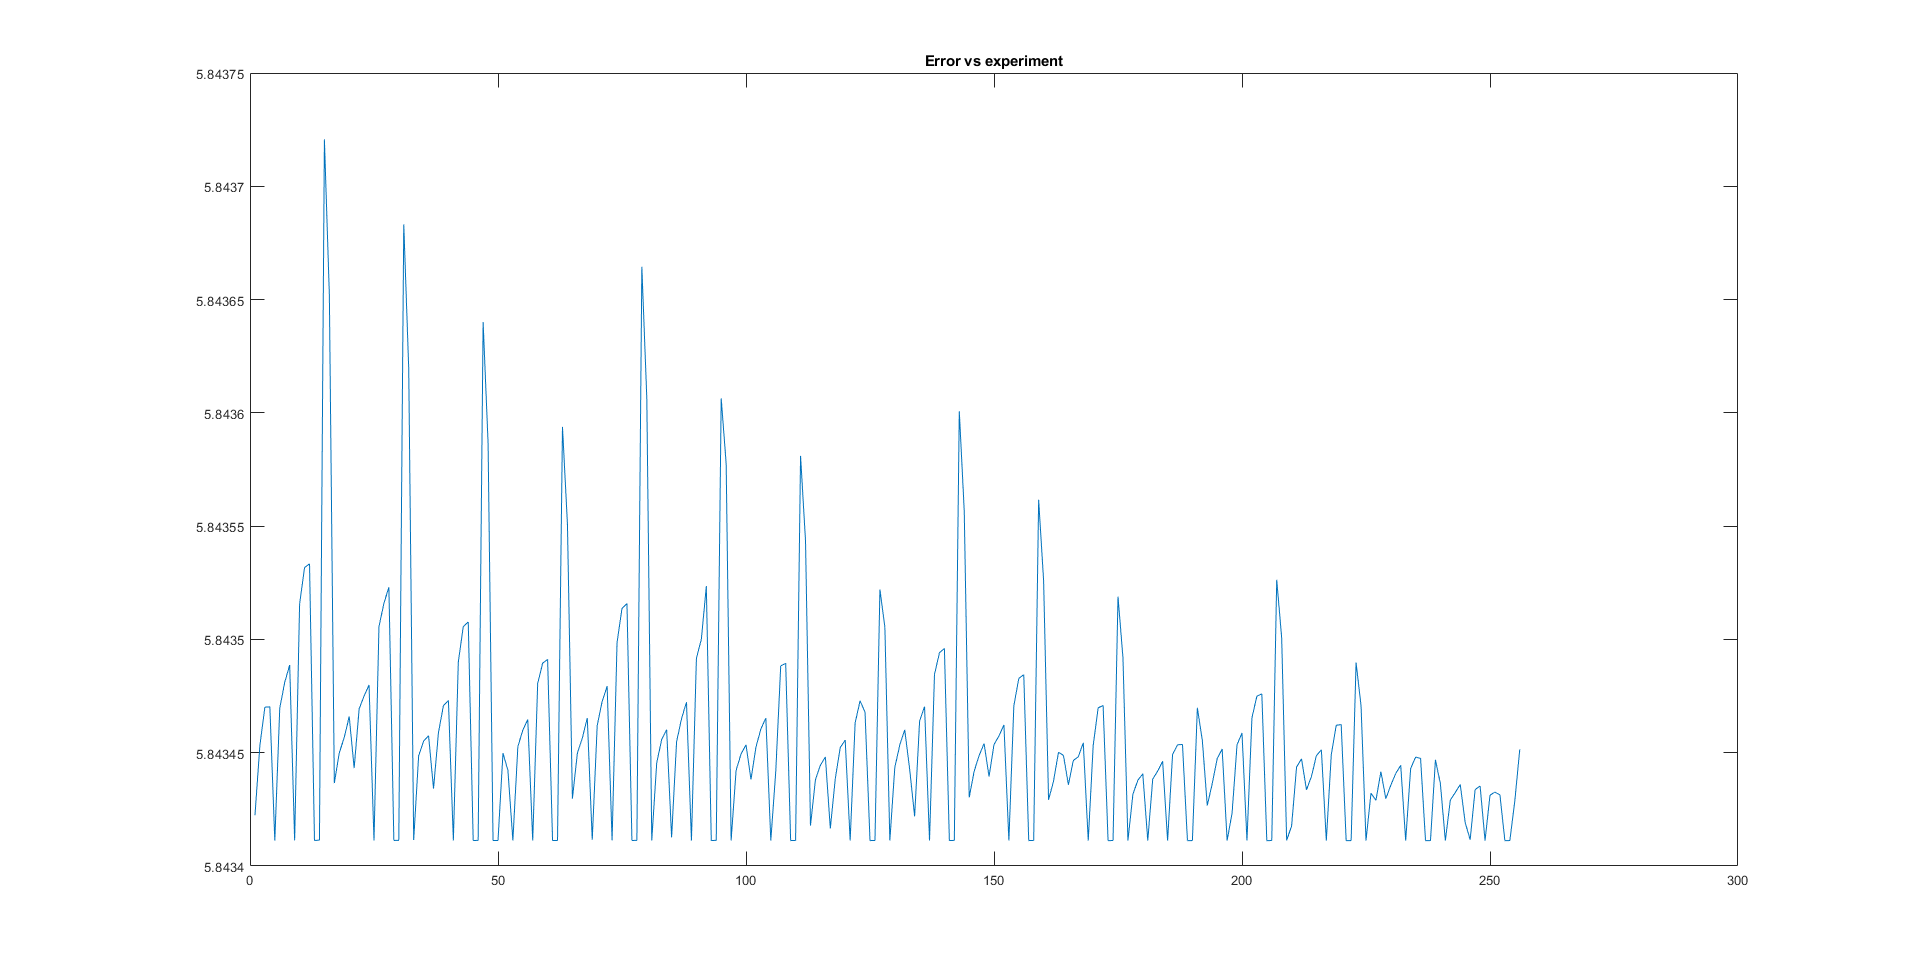
\includegraphics [width=4in]{analyze_Sensitivity_02.png}


\subsection*{Exit information for error-minimizing experiment}

\begin{verbatim}
% find error minimiizing and maximizing experiments
[error_min,min_index] = min(errors);
[error_max,max_index] = max(errors);

% - 3rd column is output of fmincon, {exitflag, output, lambda, grad, hessian};"

fminconOutput_min =  XX{min_index, 3};

exitflag_min = fminconOutput_min{1};
% xoptimal_min = fminconOutput_min{2};
gradient_min = fminconOutput_min{4};
hessian_min = fminconOutput_min{5};

%
fminconOutput_max =  XX{max_index, 3};
exitflag_max = fminconOutput_max{1};
xoptimal_max = fminconOutput_max{2};
gradient_max = fminconOutput_max{4};
hessian_max = fminconOutput_max{5};


display('Error minimizing experiment:')


display('Gradient: ')
display(gradient_min');

display('Hessian: ');
display(hessian_min);



display('Eigenvectors and eigenvalues:')
[V,D] = eig(hessian_min);
display(V)
display(diag(D))


display('Output info:')
display( fminconOutput_min{2});
\end{verbatim}

        \color{lightgray} \begin{verbatim}Error minimizing experiment:
Gradient: 
  Columns 1 through 3

     4.649162292480469e-06     2.324581146240234e-06    -9.536743164062500e-07

  Columns 4 through 6

     2.324581146240234e-06     4.172325134277344e-07    -8.344650268554688e-07

Hessian: 

hessian_min =

  Columns 1 through 3

     1.584133562547888e+02     9.467884010661443e+01    -5.288159006804295e+01
     9.467884010661443e+01     5.689752555006441e+01    -3.148548705023781e+01
    -5.288159006804295e+01    -3.148548705023781e+01     1.817475674863604e+01
     9.442857224508342e+01     5.644600499581995e+01    -3.183414691697542e+01
     1.156837602608237e+01     6.894872598905376e+00    -3.760185312335628e+00
    -4.626410448506272e+01    -2.776699436515810e+01     1.524512152373301e+01

  Columns 4 through 6

     9.442857224508342e+01     1.156837602608237e+01    -4.626410448506272e+01
     5.644600499581995e+01     6.894872598905376e+00    -2.776699436515810e+01
    -3.183414691697542e+01    -3.760185312335628e+00     1.524512152373301e+01
     5.669336129088651e+01     6.849625067351515e+00    -2.732249618718578e+01
     6.849625067351515e+00     9.143568101462891e-01    -3.301005104942880e+00
    -2.732249618718578e+01    -3.301005104942880e+00     1.402718966024112e+01

Eigenvectors and eigenvalues:

V =

  Columns 1 through 3

     3.066665006217656e-01     1.047917888826050e-01     5.907912107811094e-01
    -5.421719859765872e-02     4.068218722311226e-01    -6.834364808369163e-01
     2.380614674575998e-01    -4.775321318089210e-01     4.326855607906827e-02
    -8.993651645109052e-02    -7.088871682667939e-01    -2.910947375646066e-01
    -8.766324688707000e-01     4.538725487540422e-02     3.070455377301649e-01
     2.641397887764390e-01     3.014907761586356e-01     5.472700889013940e-02

  Columns 4 through 6

    -1.127892806118459e-01     1.073541171989333e-01    -7.222837083462943e-01
    -3.054712062266108e-01     2.905634590031494e-01    -4.321241196351137e-01
    -5.777716497848565e-01     5.667498156279628e-01     2.416447807161364e-01
    -1.011886410931777e-01    -4.565999765070766e-01    -4.311978429966635e-01
    -3.620788586527672e-01     3.630459936985886e-02    -5.253023470187956e-02
    -6.471519142217170e-01    -6.107708685068119e-01     2.109307575412916e-01

     1.238328899291367e-02
     7.780471940238935e-02
     2.142837090707748e-01
     3.490044647279442e-01
     9.927382009878066e-01
     3.034743319315812e+02

Output info:
  struct with fields:

         iterations: 19
          funcCount: 146
    constrviolation: 0
           stepsize: 4.316881058432232e-06
          algorithm: 'interior-point'
      firstorderopt: 7.078017771779683e-07
       cgiterations: 12
            message: 'Local minimum found that satisfies the constraints.↵↵Optimization completed because the objective function is non-decreasing in ↵feasible directions, to within the value of the optimality tolerance,↵and constraints are satisfied to within the value of the constraint tolerance.↵↵<stopping criteria details>↵↵Optimization completed: The relative first-order optimality measure, 7.078018e-07,↵is less than options.OptimalityTolerance = 1.000000e-06, and the relative maximum constraint↵violation, 0.000000e+00, is less than options.ConstraintTolerance = 1.000000e-06.'
       bestfeasible: [1×1 struct]

\end{verbatim} \color{black}
    

\subsection*{Plot Incidence and Prevalence of error minimizing}

\begin{verbatim}
% - 4th column is matrix, population XELTR vs time (using optimized params)
% - 5th column is TB incidence (using optimized params)

XELTR_min = XX{min_index, 4};
incidence_min = XX{min_index,5};

load('.\data and results\ReportedTB201020.mat');
figure(3)

subplot(2,1,1)
plot(Years,incidence_min(1:end-1)','r--','DisplayName','Estimated');% prevalence
hold on
plot(Years,ReportedIncidence,'k','LineWidth',2, 'DisplayName','Reported')
title('Incidence vs Time')
legend('Location','East')
hold off

subplot(2,1,2)
plot(Years,XELTR_min(1:end-1,4)','r--','DisplayName','Estimated');% prevalence
hold on
plot(Years,ReportedPrevalence,'k','LineWidth',2, 'DisplayName','Reported')
title('Prevalence vs Time')
legend('Location','East')
hold off

saveas(gcf,['Prevalence Incidence',imageName, '.png'])
\end{verbatim}

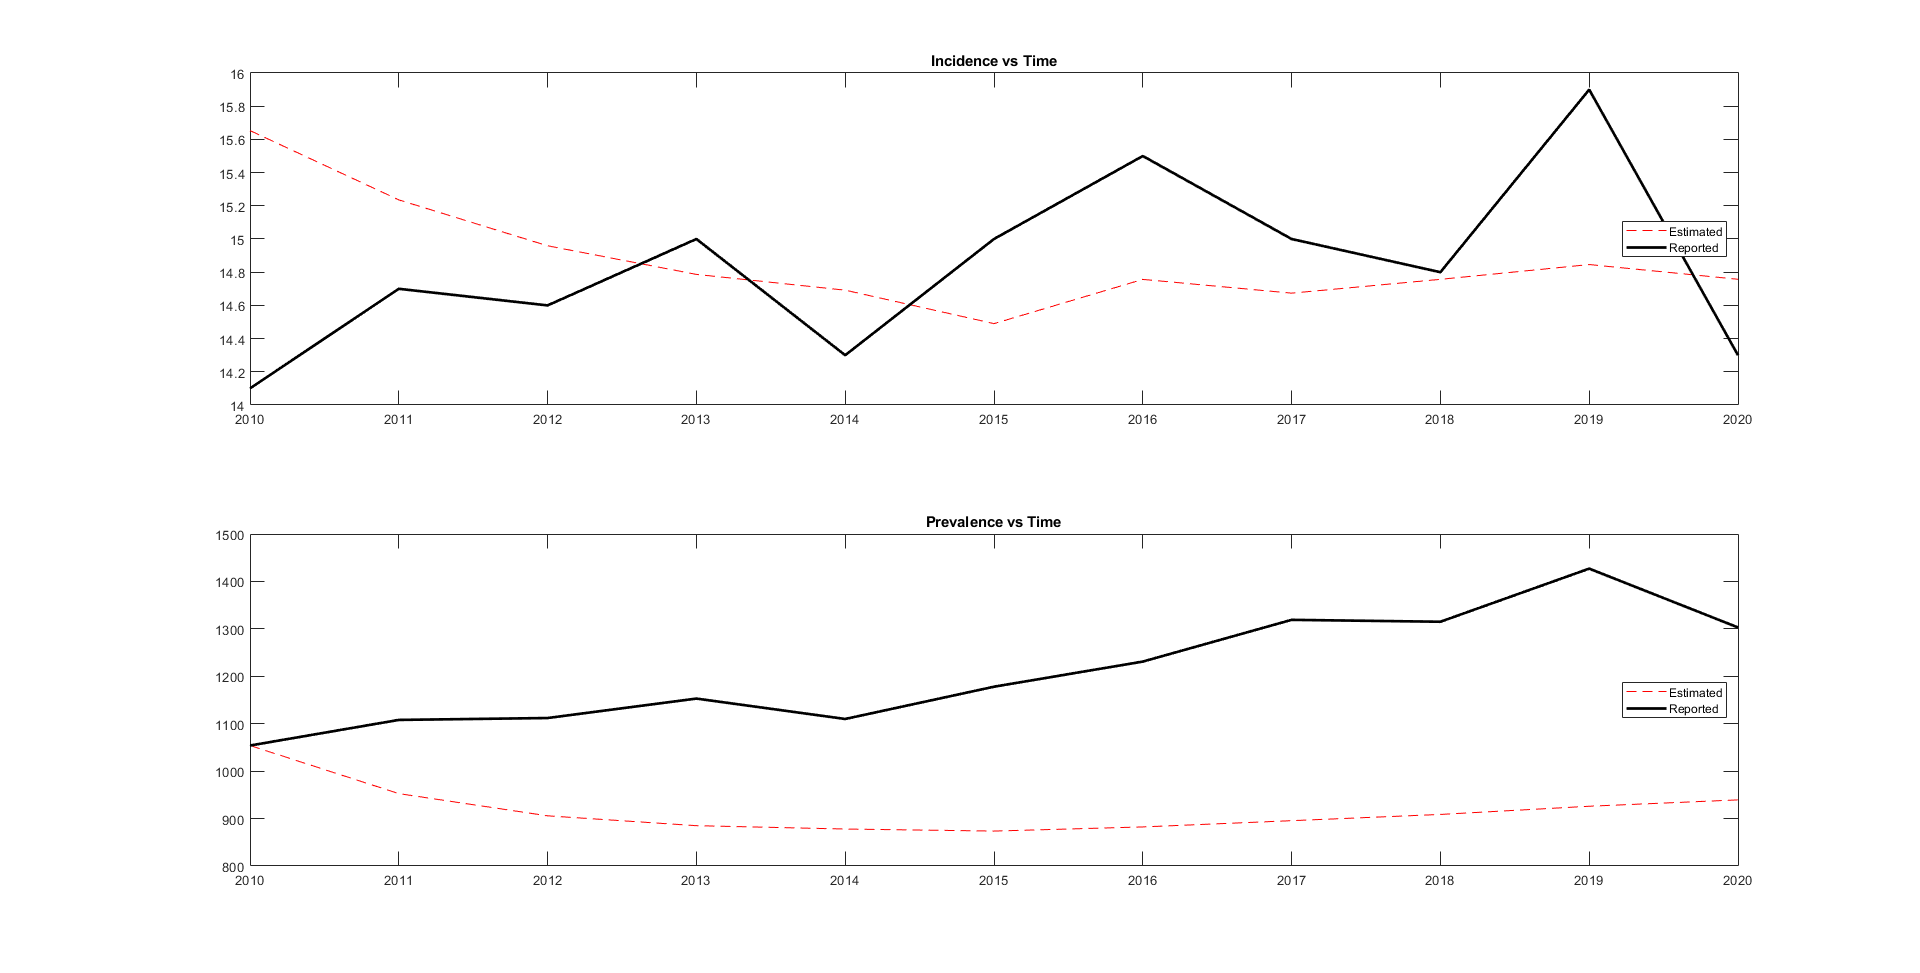
\includegraphics [width=4in]{analyze_Sensitivity_03.png}



\end{document}

